\documentclass[journal]{IEEEtran}
\usepackage{amsmath}
\usepackage{graphicx}
\usepackage{algorithm}
\usepackage{algorithmic}
\usepackage{array}
\usepackage{enumerate}
\usepackage{multirow}

\usepackage[table,x11names]{xcolor}

\usepackage{makecell}

\begin{document}

\title{Advanced Topics in Network Security}

\author{
Brant Geddes\\
Faculty of Engineering and Applied Science, University of Regina, SK, Canada S4S 0A2\\
geddes2b@uregina.ca
}

\maketitle

\begin{abstract}
There are many tradeoffs to consider when selecting encryption and key management protocols. The engineer has to consider factors such as network architecture, network resources, and the required level of security. All of these security tradeoffs additionally need to be weighed against network quality of service metrics to ensure that the network is sufficiently secure while still maintaining the required level of performance. For this reason, security protocols come in many different forms and are often highly configurable. Encryption algorithms often allow varying the key size to reduce bandwidth and processing requirements or increase the level of security provided. Exchange and management protocols can be selected from a fully centralized architecture, a fully distributed architecture, or a purpose-built hybrid architecture. These choices are often made by examining the network architecture, network size, and capabilities of the individual nodes. In addition, these decisions need to be made so that the network scales gracefully as nodes are added or removed and traffic requirements evolve. It is important to weigh all of the options carefully in order to design a network with the required performance, security, and scalability.
\end{abstract}

\begin{IEEEkeywords}
        Public Key Encryption, Elliptic-Curve Cryptography, Block Ciphers, Side-Channel Attacks, Key Exchange, Key Management
\end{IEEEkeywords}

\section{Introduction}
Security is an important topic to consider when designing a network. Security is the process of ensuring that a network and its communications cannot be compromised, faked, or altered. Information security is built on the idea of the C-I-A model:
\subsubsection{Confidentiality}
Information needs to be confidential to all outside listeners.
\subsubsection{Integrity}
The network needs to guarantee that information cannot be altered or faked in anyway.
\subsubsection{Availability}
Information needs to be available for any participants in the exchange when they need it.
\\
A network can work towards fulfilling the CIA model by selecting encryption protocols and key management protocols that meet the required level of security. Confidentiality can be met by converting plaintext messages to ciphertext using an encryption algorithm. This guarantees that an adversary eavesdropping on the message cannot read and understand the information. Integrity can be provided by authenticating messages using a key to sign them. This lets the receiver know that the message originated from the correct source and that the message content has not been tampered with. Finally, availability can be provided by selecting protocols that maintain the quality of service that the application requires.

\section{Symmetric and Asymmetric Encryption}
Two general types of encryption approaches exist, symmetric and asymmetric. Symmetric encryption depends on each participant having a shared secret. Asymmetric encryption, in contrast to symmetric, does not require a common secret between all parties. Symmetric encryption often requires less overhead but introduces the problem of how two parties share a secret key without a third party having access through eavesdropping. This problem sets the stage for a large number of key exchange algorithms for securely sharing this secret key without being at risk of eavesdropping. Asymmetric encryption does not suffer from this problem but often requires more overhead in order to generate the key and requires more storage for the key pair. Modern approaches combine the two, and public-key cryptography is often used as the key exchange method for symmetric encryption~\cite{PK1}.
\subsection{Ciphers}
Symmetric encryption is based on the use of ciphers to perform tasks such as encrypt, decrypt, sign, and verify. There are block ciphers that operate on a block of data at once, and stream ciphers that operate on streams of data continuously. Every cryptographic operation including hashing, encrypting, or more complicated functions can be built using various forms of block ciphers~\cite{BC1}~\cite{BC2}. A block cipher is often specified alongside a mode of operation to describe how the block cipher is to encrypt multiple blocks. Some examples of modes of operation are:
\begin{itemize}
        \item (ECB) Electronic Code Book
        \item (CBC) Cipher Block Chaining
        \item (CFB) Cipher Feedback
        \item (OFB) Output Feedback
        \item (CTR) Counter
\end{itemize}
Electronic Code Book operation is the simplest form and naively encrypts each block on its own. This type of encryption is not secure when used to encrypt multiple blocks, as differential analysis of the blocks could reveal the key used. An example of ECB can be seen in Figure~\ref{fig:cipher-ecb}. Other modes were created to account for the insecure nature of ECB, such as Cipher Block Chaining. CBC is a mode that fixes this problem by introducing a Initialization Vector (IV). CBC works by randomly creating an IV and using this with the key to encrypt the first block. Then the output of the first block is used as the IV for the second block and so on. Using this feedforward design allows the same key to be used in each block with a different IV, causing a different value to be used to encrypt each block. The initial IV is sent with the encrypted message, and is used to decrypt the message. An example of CBC can be seen in Figure~\ref{fig:cipher-cbc}. 
\begin{figure}[!htb]
\centerline{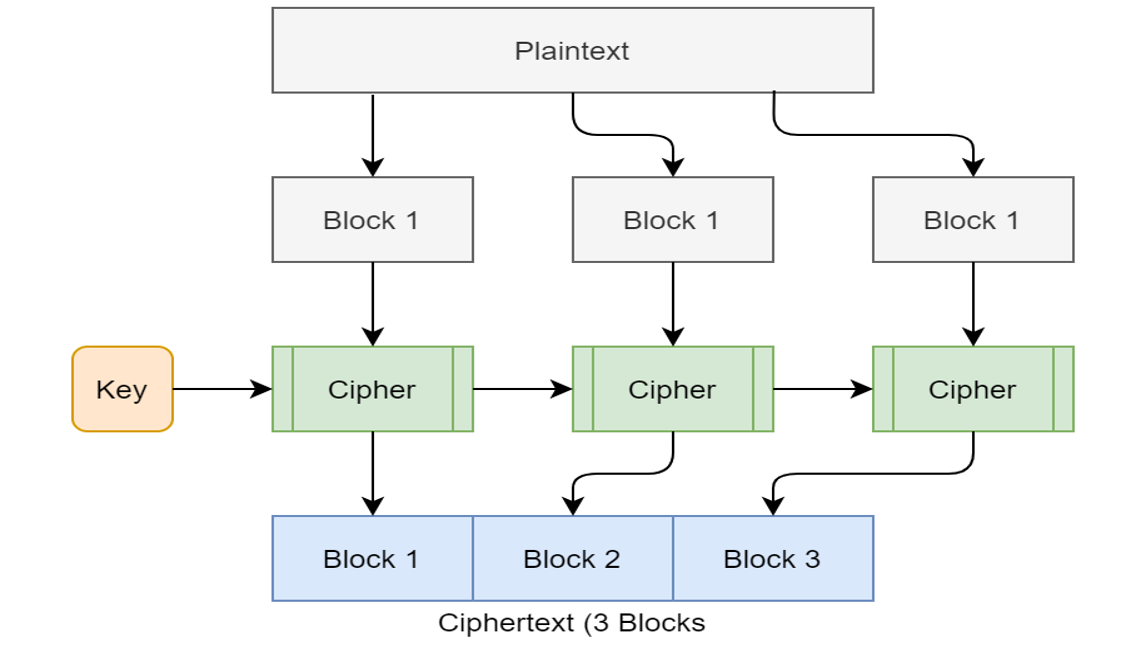
\includegraphics[totalheight=5cm]{pictures/cipher-ecb.png}}
    \caption{ECB Mode of Operation}
    \label{fig:cipher-ecb}
\end{figure}
\begin{figure}[!htb]
\centerline{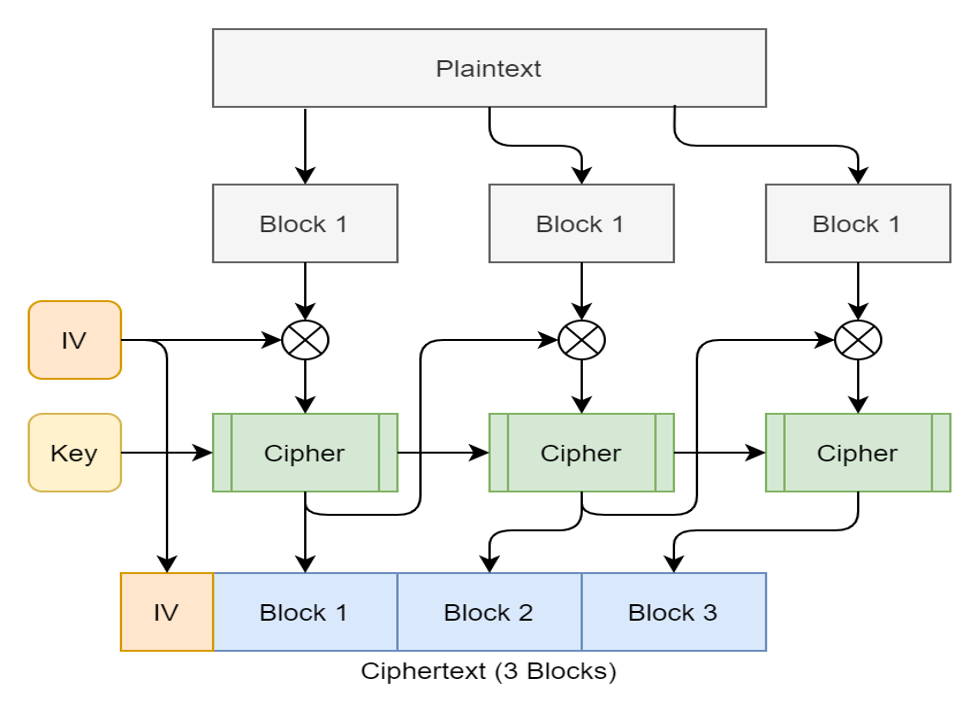
\includegraphics[totalheight=5cm]{pictures/cipher-cbc.png}}
    \caption{CBC Mode of Operation}
    \label{fig:cipher-cbc}
\end{figure}
\\
Examples of common block ciphers are the Data Encryption Standard (DES), Advanced Encryption Standard (AES), or Blowfish algorithms~\cite{BC3}. DES is able to encrypt 64-bit blocks with a key size of 56 bits. DES was found to be insecure due to the small key size and is no longer in common use. AES was designed to be used in place of DES and is able to encrypt 128-bit blocks with a key size of 128-bits, 192-bits, or 256-bits. Finally, Blowfish is another commonly used block cipher that operates on 64-bit blocks and has a key size that can range from 32-bits to 448-bits. These algorithms are used with a mode of operation to perform the various encryption operations.

\subsection{Diffie-Hellman Key Exchange}
Using block ciphers to perform symmetric encryption relies on both parties sharing a secret key. A significant problem when using symmetric algorithms is establishing the shared secret between two nodes without allowing any intermediate node to eavesdrop. One way to solve this issue is with the Diffie-Hellman (DH) key exchange. The DH algorithm allows two parties to derive a shared secret by using individual secrets and a common factor. The paint analogy seen in Figure~\ref{fig:diffie-hellman-paint} shows a simplified version of how the algorithm works.
\begin{figure}[!htb]
\centerline{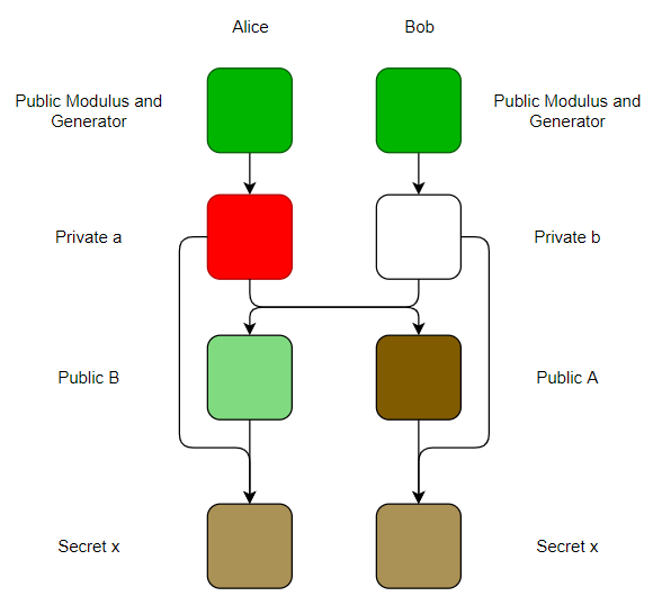
\includegraphics[totalheight=6cm]{pictures/diffie-hellman-paint.png}}
    \caption{Simplified Explanation of Diffie-Hellman Exchange}
    \label{fig:diffie-hellman-paint}
\end{figure}
The DH algorithm is based on number theory and the problem of solving logarithms over a modular field. The common factor between algorithms is a base number and a modulus. Both parties have a secret key they use for exponentiation. The following steps outline how the DH algorithm is used to derive a shared secret:
\begin{enumerate}
        \item Node A and B share common factors generator $g$ and prime modulus $p$ and generate private keys $a$ and $b$
        \item Node A generates public key $A$: $g^a(modp) = A$
        \item Node B generates public key $B$: $g^b(modp) = B$
        \item Node A and B exchange public keys $A$ and $B$
        \item Node A derives shared key $m$: $B^a(modp) = m$
        \item Node B derives shared key $m$: $A^b(modp) = m$
\end{enumerate}
After the above steps are taken, Nodes A and B share secret key $m$ after having transmitted twice and performed modular exponentiation four times.

\subsection{Shamir's Three Pass Protocol}
Shamirs Three Pass Protocol is another form of key exchange that allows two nodes to generate a shared secret key without transmitting the key as plaintext. The protocol relies on having a commutative block cipher so that when encrypting the secret multiple times with different keys, the order of decryption does not have to match the order of encryption. If \(A\) \& \(A^*\) are the encryption and decryption algorithms for node A and \(B\) \& \(B^*\) are the algorithms for node B, then the following must be true for Shamir's Three Pass Protocol to work:
\[ A^*B^*(BAm) = B^*A^*(ABm) \] 
Shamir's protocol takes the following steps to exchange the secret \(m\):
\begin{enumerate}
        \item Node A generates a secret $m$
        \item Node A encrypts secret $m$: $Am = m^*_A$
        \item Node A transmits $m^*_A$ to node B
        \item Node B receives $m^*_A$ and encrypts it again: $Bm^*_A = m^*_{AB}$
        \item Node B transmits $m^*_{AB}$ to Node A
        \item Node A decrypts $m^*_{AB}$: $A^*m^*_{AB} = m^*_B$
        \item Node A transmits $m^*_B$ to Node B
        \item Node B decrypts $m^*_B$: $B^*m^*_B = m$
\end{enumerate}
As can be seen above, node A and B are able to exchange secret $m$ without ever directly transmitting it. This allows the exchange of a secret key that is safe from eavesdropping and only requires two encryptions, two decryptions, and three transmissions.

\subsection{Rivest-Shamir-Adleman}
The Rivest-Shamir-Adleman (RSA) algorithm is an asymmetric encryption algorithm based on number theory. A node generates a pair of keys, the public key and the private key. The public key is able to encrypt a message and only the private key is able to decrypt that message. Generally, two nodes that want to communicate will generate separate key pairs, exchange public keys, then use the public keys to either exchange a shared key for symmetric encryption or use the public keys to encrypt the message itself. Security in RSA is built on the problem of solving a logarithm over a modular field. Methods exist to solve this problem in reasonable time, such as the General Number Field Sieve algorithm or certain quantum algorithms~\cite{RSA1}, so RSA keys must be made larger than an equivalent symmetric key. To achieve 112-bits of security, RSA requires a 2048-bit key~\cite{PK2}.

\subsection{Elliptic-Curve Cryptography}
Elliptic-Curve Cryptography (ECC) is a public key exchange method based on the theory of elliptic curves. This security is based on the problem of solving a discrete logarithm over a modular elliptic curve. Unlike the RSA problem, there are no known algorithms that can solve this problem easily. This means that ECC is able to deliver the same security as RSA with a smaller key size. To achieve 112-bits of security, ECC only requires a 224-bit key~\cite{PK2}. Elliptic curves are built using the following formula:
\[ y^2 = x^3 + ax + b \]
The choice of $a$ and $b$ are important~\cite{ECC1} and certain choices for curve coefficients can be solved by transforming the problem into solving a logarithm over a modular field~\cite{ECC3}, which is equivalent to solving the RSA problem. ECC algorithms specify common curve coefficients $a$ and $b$, a common starting point known as the generator point $g$, and a prime modulus $p$. ECC is based on the idea of point doubling, where the intersection of the tangent line at a point on the curve is the result of the operation. Point doubling is repeated $k$ times, where $k$ is the private key. After doubling the generator point $k$ times the public key is derived:
\[g^n = K\].
These values are used between two nodes to generate a shared secret key in an algorithm known as Elliptic-Curve Diffie Hellman (ECDH). ECDH works in the following way:
\begin{enumerate}
        \item Node A and B share common factors curve coefficients $a$ and $b$, generator $g$, and prime modulus $p$
        \item Node A and B select private keys $a$ and $b$
        \item Node A generates public key $A$: $g^a(modp) = A$
        \item Node B generates public key $B$: $g^b(modp) = B$
        \item Node A and B exchange public keys $A$ and $B$
        \item Node A derives shared key $m$: $B^a(modp) = m$
        \item Node B derives shared key $m$: $A^b(modp) = m$
\end{enumerate}
It is important to note that exponentiation in the above equations is the elliptic curve point doubling operation. Using this process, Nodes A and B are able to exchange a shared secret using two transmissions and four point doublings. The key advantage of this process is that the public keys used here are able to be much smaller than equivalent DH or RSA keys. In traditional networks this reduced key size has small advantages, such as less delay, but for constrained networks there are large benefits that can be seen by switching to ECC~\cite{ECC2}. The smaller key size corresponds to less processing time used to generate the keys, less bandwidth used when exchanging public keys, less storage used to keep keys, and less power consumption used in the whole process. Additionally, the use of ECDH allows the nodes to use cheaper symmetric encryption algorithms such as AES after the key exchange, further reducing load on the network.

\section{Methods for Breaking Encryption}
The level of security provided by certain encryption protocols can be measured using the time it would take an adversary to solve the underlying problems. For an algorithm with no known shortcuts the only solution is brute force. For example, the DES algorithm with a key size of 56-bits could take as long as $2^{56}$ operations to solve by brute force. Problems that have a shortcut, such as factoring RSA keys using the general number field sieve algorithm, are able to be solved in less operations than the brute force method. As technology advances, processors are running at higher clock speeds and are using more cores. Additionally, cloud computing has allowed tasks to be split over multiple cloud machines easily. This is the driving force behind using larger key sizes. Other than brute force or factoring algorithms, there are other methods that can be used to break encryption algorithms that do not rely on solving the underlying problem.
\subsection{Cryptanalysis}
Cryptanalysis is the field of studying encryption algorithms and breaking the algorithms using techniques that are independent of the underlying problem~\cite{CA1}. The field has two main techniques: 
\subsubsection{Linear Cryptanalysis}
Linear cryptanalysis attempts to recover the key used when encrypting by building the following system of equations:
\[ P_i \otimes K = C_i \]
Where $P_i$ is the plaintext message, $C_i$ is the corresponding ciphertext message, and $K$ is the key used to encrypt. By solving a system of plaintext-ciphertext pairs, the key can be recovered. The more of the message pairs that the adversary obtains, the easier this task is. This is one reason why keys should be renewed often. The main defense against linear cryptanalysis is to introduce non-linear elements in the encryption process, which make the system of equations much more difficult to solve.
\subsubsection{Differential Cryptanalysis}
Differential cryptanalysis recovers plaintext from ciphertext by studying many ciphertext messages encrypted with the same key and attempting to link differences in the output to differences in the input. If the same key is used to encrypt every message, an adversary can often recover plaintext from ciphertext using this method. The main defense against this method is to use a more advanced mode of operation such as CBC that mixes using a constant key with a different initialization vector for each block. 
\subsection{Side-Channel Attacks}
Another method for bypassing security besides solving the encryption problem or performing cryptanalysis is to attack side-channels in the encryption process. Side-channels are additional attack vectors other than the ciphertext and key that can be examined to recover information. Side-channels include:
\subsubsection{Power Differential}
Power differential attacks look at power consumption of the processor while it is performing encryption and analyse the difference between the baseline power consumption and spikes seen while encrypting~\cite{SC1}. This can reveal factors such as the key size, value, or even the plaintext message that was encrypted.
\subsubsection{Timing}
Timing attacks measure the time taken to encrypt certain inputs and use the time along with the output to attempt to reveal the key used~\cite{SC2}. Timing attacks use the fact that certain instructions can take more time to process, such as branching, cache hits and misses, pipeline bubbling, or any processor optimizations. These differences can reveal patterns that help the adversary recover the key.
\subsubsection{Cache}
Cache attacks are attacks that attempt to recover sensitive information from the processor cache by tricking the processor into storing information in the cache~\cite{SC4}. A modern example is the Spectre attack~\cite{SC3}. Spectre is a combination timing/cache attack that uses a processor optimization known as speculative execution to have the processor store sensitive information in the cache. Speculative execution is an optimization that has a processor pre-compute values while it is idle. Using the Spectre attack, an adversary is able to force the processor to pre-compute sensitive information and store it in the cache before the processor knows that the currently running process does not have access to the information.
\subsubsection{Electromagnetic Leakage}
Electromagnetic leakage attacks are similar to power differential attacks, but instead of requiring direct access to the machine to measure power consumption, an antenna is used to measure electromagnetic radiation. EM levels vary with current and voltage, so spikes in power consumption generally correspond to spikes in EM radiation. In ~\cite{SC5}, Zajić and Prvulovic show that they are able to use this attack to read EM radiation from an i7 processor from as far as 1.6 meters using a laptop and antenna. The time-series EM radiation data can be used in the same way the power differential information is used to recover sensitive information.
\subsubsection{Fault}
Another side-channel that adversaries are able to attack are system faults. By introducing faults in a system an attacker can gain valuable information or gain access to the system. An example of a fault attack against a common RSA implementation known as Duursma-Lee can be seen in ~\cite{SC6}. This attack introduces a fault that changes the bounds of the algorithm, allowing the attacker to obtain the private key. Another common example of a fault attack is known as buffer overflow. A buffer overflow attack attempts to write malicious code into the memory of the system by overflowing an input variable. If the target system does not check bounds on the input, an adversary can write code that overflows into the systems code space and is executed. This code can be written to provide the attacker access to the system.

\section{Key Management}
Another important topic in security is key management. Encryption protocols and key exchange protocols work well for pairs of nodes, but in larger systems it is often helpful to define an overall key management protocol to reduce the work required by individual nodes. Without a key management protocol a node is responsible for performing this operation with every other node it may need to communicate with. This grows exponentially as the network size increases, causing problems when concepts such as key renewal are taken into account. For that reason, several management protocols have been designed to help with this problem.
\subsection{Distributed}
A distributed key management concept is one where the individual nodes are responsible for managing keys. This can be as simple as each node performing a key exchange with its neighbors in small networks to key pairs being pre-defined on each node before the network is implemented. Distributed management protocols are typically low cost and quick, but scale very poorly as the network grows. Eventually a distributed protocol will fail if the network becomes large enough.
\subsection{Centralized}
Centralized key management is a concept where a central agent manages keys for the network. Using this system, each node only needs to perform an exchange with the central authority. When two nodes need to communicate, they ask the central authority for the keys needed. This system is commonly used with the Secure Hypertext Transport Protocol (HTTPS) protocol where a client uses a certificate issued by a third-party Certificate Authority (CA) to verify the authenticity of the server it is trying to connect to. This works well for conventional networks, but in more constrained networks there are downsides to using this system. A large disadvantage is that the CA has a large load put on it by the rest of the network and generally needs to be more powerful, have larger storage, and have a larger energy capacity. Another disadvantage, is that this provides a single point of failure for the network. If the CA is compromised or goes offline the whole network is unable to communicate until the CA is repaired.
\subsection{Hybrid}
Hybrid key management shares concepts of both distributed and centralized management. It is often based on a tree architecture where cluster heads are the CAs for only their clusters. This reduces the effect of losing a CA as only that cluster is affected and the rest of the network is able to continue working. It also helps alleviate the issue of the load put on a single node acting as a CA as this load is shared across multiple cluster heads. Hybrid management systems also have the advantage of being able to be tailored for a specific use case. An example of tailoring a hybrid protocol for a use case is seen in ~\cite{KM2}, where the authors build a secure, cluster-based system for exchanging and managing keys in a medical application. The system is based on the theory of elliptic curves, and provides an easily generated shared session key that can be used to establish a secure session. This session key is used once and then discarded to improve security. The authors optimized the exchange to put as little stress on the cluster members as possible and shift most of the work to the cluster heads. Other examples of building hybrid key management protocols can be seen in ~\cite{KM1}, where the authors use routing information to define specialized clusters, and ~\cite{KM3}, where the authors use deployment information to define neighborhoods where keys are shared.

\section{Conclusion}
There is a significant challenge when designing and implementing any network due to the need to balance several competing metrics. Power consumption, bandwidth, delay, and security are all dependant on each other and focusing on one will often cause the others to suffer. Thankfully, there are many options to choose from when implementing a security suite that often enable a designer to balance quality of service metrics with security requirements. In traditional wired networks, the RSA algorithm or DH key exchange are able to deliver an adequate amount of security while allowing the network to perform normally. Concepts such as centralized key management and exchange allow more powerful nodes in the cloud (Certificate Authorities) to handle the bulk of the security overhead. In more constrained networks there are optimizations available to help reduce this overhead. ECC has proven to be a powerful option as it is able to perform at the same level of security as RSA with a smaller key size. This helps reduce everything from processing power required for key derivation, network bandwidth for key sharing, and storage space for keeping the keys. This reduced load required to work with an ECC protocol means that the network experiences reduced overhead and can perform expensive operations like refreshing keys more often. Finally, constrained networks have the option of using hybrid key management schemes to better fit the needs of the network. In extremely tight designs with harsh targets, it is often possible to design a specialized hybrid protocol that meets the required security while working with the network to maintain the target quality of service. In conclusion, there are many security options available for use in modern network design. However there are significant tradeoffs involved and a design must balance the various metrics carefully.
\vspace{25mm}
\bibliographystyle{IEEEtran}
\bibliography{references}

\end{document}
